\documentclass[10pt,a4paper]{article}
\usepackage[utf8]{inputenc}
\usepackage{amsmath}
\usepackage{geometry}
\usepackage{amsfonts}
\usepackage{amssymb}
\usepackage{subcaption}
\usepackage{titling}
\usepackage{listings}
\usepackage[
backend=bibtex,
style=science,
sorting=none
]{biblatex}

\usepackage[english]{babel}
\usepackage{graphicx}

\begin{document}

\begin{titlingpage}
\title{Tidal Tails}
\author{Candidate Number: 6892V}
\maketitle
\begin{abstract}
This program provides an interactive simulation and visualisation of the effects a perturbing galaxy can have on test particles that are initially following a circular orbit around a stationary central mass. It can also function as a general interactive N-body simulator if the appropriate launch time flag is chosen. This report investigated the forming of elongated streams of particles (tidal tails) as perturbing galaxies pass by the central mass. Tidal tails are seen to form when appropriate orbits of the perturbing galaxy are chosen. Various parabolic orbits with different distances of closest approach were visualised, for each of these orbits both clockwise and anticlockwise initial rotations of the test particles were simulated. It was seen that tidal tails were most pronouncedly formed if the test particles followed an initially anticlockwise orbit and the perturbing galaxy had a closest approach just outside the outer ring of test particles.
\end{abstract}
	
\end{titlingpage}

\clearpage
\section{Introduction}
The aim of this project is to simulate/observe the creation of tidal tails. Tidal tails are created when two galaxies pass one another and interact gravitationally. A tidal tail is an elongated stream of stars that extends outwards from a galaxy.  To do this an N-body simulation of massive particles was created using C++, and visualised using SDL2/OpenGL. To observe the formation of tidal tails a galaxy with a fixed central mass was created, test particles were then set in motion in a uniform distribution around this central mass such that the orbits were circular. A perturbing galaxy was then introduced on several different orbits (conic sections) with various input parameters. Tidal tail formation was observed and the results were screenshotted at various times after introduction for each of these orbits. 
\\
\\
The computational techniques used in this program will be analysed in section 2, following this the specific implementation and how the simulation performed will be discussed in section 3. The screenshots of the Tidal Tails and discussions of them will be contained in section 4. And finally any concluding remarks will be in section 5. An appendix containing instructions and full code listings is included at the end of this document. 
\\
\\
The program created is interactive the camera can move around the scene, screenshots can be taken, logging can be toggled on/off and if the correct flag is activated (INTERACTIVE) masses can be created by clicking. The input parameters for the perturbing galaxy can be set using command line arguments when starting the program. In the simulation the central mass and perturbing galaxy are green in colour, the test particles are red and the trail of the perturbing galaxy is blue. Detailed instructions on how to operate this program are provided in section 6.
\\
\\
The aim of this program was to find out how the direction of rotation of the test particle's initial orbits affect the formation of tidal tails for various perturbing galaxies with parabolic trajectories.

\clearpage
\section{Analysis of Methods}
First of all the problem required scaling, in typical units (SI) the gravitational constant $G=6.67\times10^{-11} m^3 kg^{-1} s$ and a typical central mass might be many orders of magnitude larger than the mass of the sun ($M_\odot=2.0\times10^{30 } kg$). Units where G = 1 and the central mass M = 1 were selected (the perturbing galaxy also defaults to having a mass of 1). This scaling is required because otherwise we would have time scales of orbits which are far too long to simulate, and smaller values are in general easier to deal with.
\\
\\
Another issue is the potential for infinities to arise in simulations. These infinities arise due to the singular nature of the gravitational force at small distances. To compensate for this the force on a test particle after entering the surface of a large mass was altered to a repulsive radial force $(\frac{GM}{r^2} \underline{\hat{r}})$. In this way a particle can't penetrate far enough in to a particle for infinities to arise. This method provides a crude simulation of collisions between the test particles and large masses.
\\
\\
A Verlet integration method was selected for this simulation in part because it is symplectic (unlike RK4) which means it will conserve energy well, this is very important in orbital dynamics to prevent energy drift and to maintain stable orbits. Another reason it was chosen is due to it being only slightly more computationally expensive than other lower order methods (euler) while having errors of order $\Delta t^4$ rather than $\Delta t^2$. Verlet is also less computationally expensive than RK4. Finally implementing an integrator using Verlet rather than RK4 meant that the acceleration only needed to be evaluated at the particle's current position. The Verlet algorithm requires current and past information only and doesn't depend on predicting future values like RK4. This means Verlet lends itself well to the "real-time" visualisation that this program intends to achieve.
\\
\\
OpenGL/SDL2 were selected to visualise the formation of tidal tails over traditional graphing solutions. This decision was made so that the simulation could be interactive (move around zoom in/out) and also so that tidal tails could be observed continuously and screenshotted during formation in "real time".
\\
\\
The suggested dark matter halo form of the perturbing galaxy (from Project Manual) can easily be implemented by setting the radius of the perturbing galaxy to a size comparable to the central mass plus its test particles and modifying the force function for test particles inside the perturbing galaxy's radius to be the same as for the inside of a uniform spherical mass. $\underline{F} \propto -|\underline{r}_{galaxy}-\underline{r}_{test}|$.
\clearpage
\section{Implementation and Performance}
The first implementation issue was to decide the integrator to use, Verlet was selected. The Verlet algorithm is as follows 
\begin{equation}
	\underline{x}_{n+1} = 2 \underline{x}_n - \underline{x}_{n-1} + \frac{1}{2}  \underline{a}(\underline{x}_n) {\Delta t }^ 2 .
\end{equation}  
This obviously requires the particle's previous and current position to calculate the particle's next position. At t = 0 we only know the particle's current position so the first time step must be carried out using a different algorithm. A simple 2nd order method was selected to carry out the first time step, $\underline{x}_{1} =  \underline{x}_0 + \underline{v}_0 {\Delta t} + \frac{1}{2}  \underline{a}(\underline{x}_0) {\Delta t }^ 2 .$ All future steps were then carried out using the Verlet algorithm. A time step of 0.005s was chosen for use in the Verlet algorithm because it was the smallest precision that didn't affect the smoothness of the visualisation.
\\
\\
The algorithm was tested using circular orbits to determine that it was functioning correctly. The radius of the orbit was plotted as a function of time for several orbits to determine the degree of variation. An example plot is shown in Figure ~\ref{fig:fig}. 
\begin{figure}[ht!]
\centering
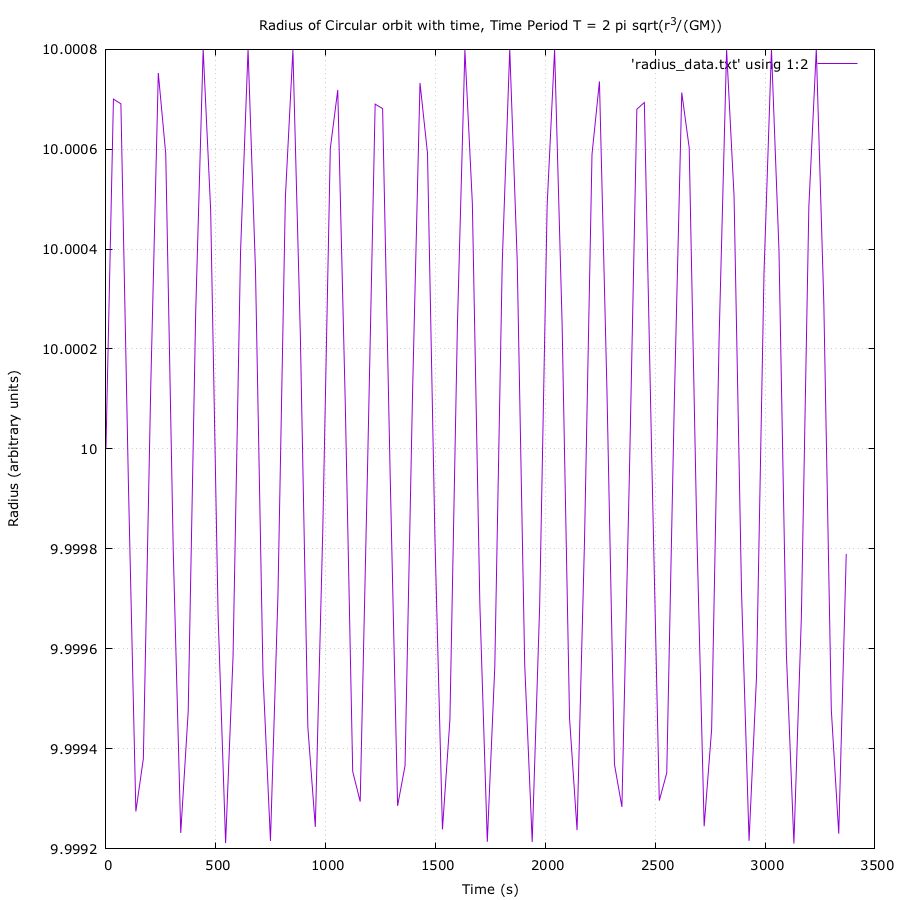
\includegraphics[width=80mm, height=40mm]{../output/Radius.png}
\caption{The variation in radius for a test mass in a circular orbit at a radius of 10 (units), shows small sinusoidal variations around the initial radius. The graph shows roughly 18 orbits.
\label{fig:fig}}
\end{figure}
\\
The radius shows small order variations, indicating the algorithm was functioning as intended. Testing can be turned on by setting the TESTING flag to true. Orbits for many test particles were observed over many cycles to make sure they were following the expected trajectories (conic sections). These were tested by modifying the galaxy creation step in the orbit\_test function in the main.cpp file.
\\
\\
The loops that determine the accelerations of each of the particles only loop over the particles that are massive, this helps to speed up the computation by removing unnecessary loops. The test particles can be given mass by setting a flag but this results in the breakdown of the galaxies structure over time and also increases the computation time. These effects are undesirable so the test particles were assigned 0 mass. Another optimisation that was used was to store any vectorial quantities (position, velocity, acceleration) in fixed sized arrays of length 3 which are often more efficient to use than dynamic sized ones. These arrays are 3D so that the program is most general, but they can easily be reduced to 2D by changing the typedef statement of vec3 in the utilities.cpp source file. The results would not change as the visualisation and initial conditions are all in the x-y plane only. This reduction in dimension would reduce the memory footprint of each particle object. But the performance is satisfactory in the general 3D case, so 3D arrays were used.
\\
\\
Performance was monitored to determine any possible causes of slow down. By turning off the rendering portion of the program and logging to data files instead it was seen that most of the computation time was in fact being used to render the particles to the screen after each time step. To reduce the time taken rendering particle motion was only rendered after a certain amount of CPU time had passed and not after every time step. Doing this resulted in a much smoother visualisation and allowed the simulation to run much closer to real time. The method  was adaptive in that the number of frames rendered each second scaled with the number of particles in the system, meaning larger systems are rendered less often. This helps to prevent the visualisation from slowing to a crawl.
\\
\\
Finally tests were carried out to determine the maximum amount of test particles that could be created without slowing the visualisation too much. With around 8000 test particles the simulations can be completely visualised within a few of minutes (2-5). This is a reasonable time for visualisation, so approximately 8000 test particles  were included. The distributions of these particles were set according to the project manual's guidelines but with many more particles per ring.
\\
\\
The program was created with object orientation in mind. Four classes were created. A particle class which housed all information about each individual particle and provided a function to render the particle. A universe class which housed pointers to all of the particles in a system, contained functions to generate galaxies, and functions that handled updating particle locations and logging of particle data. A logger class which essentially acted as a data logging device and stored particle positions in a data file when requested. And finally a camera class which stored the camera's location and calculated the zoom factor of the view, these quantities are then used during rendering to project the correct image of the scene on to the screen.
\\
\\
To simplify the determination of the initial conditions of the system (for a conic orbit) the central galaxy's central mass was fixed at the origin (0,0,0). Choosing a system like this makes it very easy to introduce a perturbing galaxy that orbits in a conic section. The initial conditions for these orbits are quite straightforward to determine using the standard results for conic sections.

\begin{enumerate}
\item $E_{total} = -\frac{G M_1 M_2}{2 a} =\frac{1}{2} M_1 \underline{v}_1^2 + \frac{1}{2} M_2 \underline{v}_2^2 -\frac{G M_1 M_2}{|\underline{r}_1-\underline{r}_2|}$
\item Semi major axis $a = \frac{r_{min}}{1-e}$
\item Polar equation of conic section $r = \frac{(1+e)r_{min}}{1+e\cos{\theta}}$
\item Cartesian coordinates $x=r\cos{\theta},y=r\sin{\theta}$
\end{enumerate}

Combining equation 1 and 2 and using the fact that the central mass (subscript 1) is fixed with 0 velocity at the origin it is possible to find the magnitude of the initial velocity of the perturbing galaxy. To find the direction of the velocity you can use the fact that the velocity vector must be a tangent to the galaxy's orbit. Rewriting equation 3 in Cartesian form and finding $\frac{dy}{dx}$ it is possible to determine this tangent vector. To find the perturbing galaxy's initial position you just need to convert the polar form of the orbit (3) into Cartesian coordinates using (4). To specify these initial coordinates and velocity we need 3 independent parameters the eccentricity e, the starting angle $\theta_0$, and the distance of closest approach $r_{min}$. These 3 quantities are taken as input parameters in the program and are used to determine the initial conditions for the perturbing galaxy.

\clearpage
\section{Results and Discussion}
Multiple parabolic perturbing orbits were simulated. Images at various time slices for each orbit are provided below. The appropriate command line arguments to recover the plots are provided in the corresponding figure caption. The closest approach of the perturbing galaxy was varied over the range 2-18 units and for each of these approach parameters both clockwise $\circlearrowright$ and anticlockwise $\circlearrowleft$ rotation (of the test particles around the central mass) were simulated. It seems that the tidal tails become most pronounced when the perturbing galaxy has its closest approach just outside the farthest out ring of test particles. From the images included we also see that if the test particles are set in motion such that they move in the same direction as the perturbing galaxy (clockwise) then the structure of the initial orbit seems to break and pronounced tail formation does not happen. However if the test particles move against the direction of the perturbing galaxy's orbit (anticlockwise) then the structure of the initial orbits can still be seen and tidal tail formation is much more pronounced.

\section{Conclusion}
This program provides the means to simulate the effects the different types of orbit of a perturbing galaxy can have on a stationary test galaxy. It is seen in the images provided that parabolic perturbing galaxies can produce tidal tails, with the exact shape of the parabola and rotation direction of the test particles determining the overall shape of any tidal tails. The program could be improved by implementing a more accurate model of the perturbing galaxy, currently the perturbing galaxy interacts with the test particles as if it were just a small solid sphere. A possible improvement could be implementation of the dark matter halo form of a galaxy suggested by the project manual (easily implemented in the current program by setting the radii of the galaxies to large values, and altering the force function). The visualisation proved quite successful as it provided the means to observe the origin and continuous formation of the tidal tails. Overall the program successfully manages to simulate the formation of tidal tails provided appropriate input parameters are chosen.

\clearpage
\begin{figure}
\begin{subfigure}{.5\textwidth}
  \centering
  \includegraphics[width=.8\linewidth]{{../output/e-rmin-theta0-rot-1-2-0.35--1/screenshot-5.00_(-15.00_15.00)(-15.00_15.00)}.png}
  \caption{t = 5.0s}
  \label{fig1:sfig1}
\end{subfigure}%
\begin{subfigure}{.5\textwidth}
  \centering
  \includegraphics[width=.8\linewidth]{{../output/e-rmin-theta0-rot-1-2-0.35--1/screenshot-10.00_(-15.00_15.00)(-15.00_15.00)}.png}
  \caption{t = 10.0s}
  \label{fig1:sfig2}
\end{subfigure}
\begin{subfigure}{.5\textwidth}
  \centering
  \includegraphics[width=.8\linewidth]{{../output/e-rmin-theta0-rot-1-2-0.35--1/screenshot-15.00_(-15.00_15.00)(-15.00_15.00)}.png}
  \caption{t = 15.0s}
  \label{fig1:sfig3}
\end{subfigure}
\begin{subfigure}{.5\textwidth}
  \centering
  \includegraphics[width=.8\linewidth]{{../output/e-rmin-theta0-rot-1-2-0.35--1/screenshot-20.00_(-15.00_15.00)(-15.00_15.00)}.png}
  \caption{t = 20.0s}
  \label{fig1:sfig4}
\end{subfigure}
\begin{subfigure}{.5\textwidth}
  \centering
  \includegraphics[width=.8\linewidth]{{../output/e-rmin-theta0-rot-1-2-0.35--1/screenshot-25.00_(-15.00_15.00)(-15.00_15.00)}.png}
  \caption{t = 25.0s}
  \label{fig1:sfig5}
\end{subfigure}
\begin{subfigure}{.5\textwidth}
  \centering
  \includegraphics[width=.8\linewidth]{{../output/e-rmin-theta0-rot-1-2-0.35--1/screenshot-30.00_(-15.00_15.00)(-15.00_15.00)}.png}
  \caption{t = 30.0s}
  \label{fig1:sfig6}
\end{subfigure}
\caption{Plots at 6 different times (30 units x 30 units) for a perturbing galaxy with a parabolic orbit (e = 1) of closest approach 2 units and starting angle $0.35 \times 2\pi$. Test particles initially in clockwise circular orbit around central mass. (cmd-line args \{1 0.35 2 -1 1\}) }
\label{fig1:fig1}
\end{figure}
\clearpage

\begin{figure}
\begin{subfigure}{.5\textwidth}
  \centering
  \includegraphics[width=.8\linewidth]{{../output/e-rmin-theta0-rot-1-2-0.35-1/screenshot-5.00_(-15.00_15.00)(-15.00_15.00)}.png}
  \caption{t = 5.0s}
  \label{fig2:sfig1}
\end{subfigure}%
\begin{subfigure}{.5\textwidth}
  \centering
  \includegraphics[width=.8\linewidth]{{../output/e-rmin-theta0-rot-1-2-0.35-1/screenshot-10.00_(-15.00_15.00)(-15.00_15.00)}.png}
  \caption{t = 10.0s}
  \label{fig2:sfig2}
\end{subfigure}
\begin{subfigure}{.5\textwidth}
  \centering
  \includegraphics[width=.8\linewidth]{{../output/e-rmin-theta0-rot-1-2-0.35-1/screenshot-15.00_(-15.00_15.00)(-15.00_15.00)}.png}
  \caption{t = 15.0s}
  \label{fig2:sfig3}
\end{subfigure}
\begin{subfigure}{.5\textwidth}
  \centering
  \includegraphics[width=.8\linewidth]{{../output/e-rmin-theta0-rot-1-2-0.35-1/screenshot-20.00_(-15.00_15.00)(-15.00_15.00)}.png}
  \caption{t = 20.0s}
  \label{fig2:sfig4}
\end{subfigure}
\begin{subfigure}{.5\textwidth}
  \centering
  \includegraphics[width=.8\linewidth]{{../output/e-rmin-theta0-rot-1-2-0.35-1/screenshot-25.00_(-15.00_15.00)(-15.00_15.00)}.png}
  \caption{t = 25.0s}
  \label{fig2:sfig5}
\end{subfigure}
\begin{subfigure}{.5\textwidth}
  \centering
  \includegraphics[width=.8\linewidth]{{../output/e-rmin-theta0-rot-1-2-0.35-1/screenshot-30.00_(-15.00_15.00)(-15.00_15.00)}.png}
  \caption{t = 30.0s}
  \label{fig2:sfig6}
\end{subfigure}
\caption{Plots at 6 different times (30 units x 30 units) for a perturbing galaxy with a parabolic orbit (e = 1) of closest approach 2 units and starting angle $0.35 \times 2\pi$. Test particles initially in anticlockwise circular orbit around central mass. (cmd-line args \{1 0.35 2 1 1\}) }
\label{fig2:fig2}
\end{figure}
\clearpage

\begin{figure}
\begin{subfigure}{.5\textwidth}
  \centering
  \includegraphics[width=.8\linewidth]{{../output/e-rmin-theta0-rot-1-6-0.2--1/screenshot-5.00_(-15.00_15.00)(-15.00_15.00)}.png}
  \caption{t = 5.0s}
  \label{fig3:sfig1}
\end{subfigure}%
\begin{subfigure}{.5\textwidth}
  \centering
  \includegraphics[width=.8\linewidth]{{../output/e-rmin-theta0-rot-1-6-0.2--1/screenshot-10.00_(-15.00_15.00)(-15.00_15.00)}.png}
  \caption{t = 10.0s}
  \label{fig3:sfig2}
\end{subfigure}
\begin{subfigure}{.5\textwidth}
  \centering
  \includegraphics[width=.8\linewidth]{{../output/e-rmin-theta0-rot-1-6-0.2--1/screenshot-15.00_(-15.00_15.00)(-15.00_15.00)}.png}
  \caption{t = 15.0s}
  \label{fig3:sfig3}
\end{subfigure}
\begin{subfigure}{.5\textwidth}
  \centering
  \includegraphics[width=.8\linewidth]{{../output/e-rmin-theta0-rot-1-6-0.2--1/screenshot-20.00_(-15.00_15.00)(-15.00_15.00)}.png}
  \caption{t = 20.0s}
  \label{fig3:sfig4}
\end{subfigure}
\begin{subfigure}{.5\textwidth}
  \centering
  \includegraphics[width=.8\linewidth]{{../output/e-rmin-theta0-rot-1-6-0.2--1/screenshot-25.00_(-15.00_15.00)(-15.00_15.00)}.png}
  \caption{t = 25.0s}
  \label{fig3:sfig5}
\end{subfigure}
\begin{subfigure}{.5\textwidth}
  \centering
  \includegraphics[width=.8\linewidth]{{../output/e-rmin-theta0-rot-1-6-0.2--1/screenshot-30.00_(-15.00_15.00)(-15.00_15.00)}.png}
  \caption{t = 30.0s}
  \label{fig3:sfig6}
\end{subfigure}
\caption{Plots at 6 different times (30 units x 30 units) for a perturbing galaxy with a parabolic orbit (e = 1) of closest approach 6 units and starting angle $0.2 \times 2\pi$. Test particles initially in clockwise circular orbit around central mass. (cmd-line args \{1 0.2 6 -1 1\}) }
\label{fig3:fig3}
\end{figure}
\clearpage

\begin{figure}
\begin{subfigure}{.5\textwidth}
  \centering
  \includegraphics[width=.8\linewidth]{{../output/e-rmin-theta0-rot-1-6-0.2-1/screenshot-5.00_(-15.00_15.00)(-15.00_15.00)}.png}
  \caption{t = 5.0s}
  \label{fig4:sfig1}
\end{subfigure}%
\begin{subfigure}{.5\textwidth}
  \centering
  \includegraphics[width=.8\linewidth]{{../output/e-rmin-theta0-rot-1-6-0.2-1/screenshot-10.00_(-15.00_15.00)(-15.00_15.00)}.png}
  \caption{t = 10.0s}
  \label{fig4:sfig2}
\end{subfigure}
\begin{subfigure}{.5\textwidth}
  \centering
  \includegraphics[width=.8\linewidth]{{../output/e-rmin-theta0-rot-1-6-0.2-1/screenshot-15.00_(-15.00_15.00)(-15.00_15.00)}.png}
  \caption{t = 15.0s}
  \label{fig4:sfig3}
\end{subfigure}
\begin{subfigure}{.5\textwidth}
  \centering
  \includegraphics[width=.8\linewidth]{{../output/e-rmin-theta0-rot-1-6-0.2-1/screenshot-20.00_(-15.00_15.00)(-15.00_15.00)}.png}
  \caption{t = 20.0s}
  \label{fig4:sfig4}
\end{subfigure}
\begin{subfigure}{.5\textwidth}
  \centering
  \includegraphics[width=.8\linewidth]{{../output/e-rmin-theta0-rot-1-6-0.2-1/screenshot-25.00_(-15.00_15.00)(-15.00_15.00)}.png}
  \caption{t = 25.0s}
  \label{fig4:sfig5}
\end{subfigure}
\begin{subfigure}{.5\textwidth}
  \centering
  \includegraphics[width=.8\linewidth]{{../output/e-rmin-theta0-rot-1-6-0.2-1/screenshot-30.00_(-15.00_15.00)(-15.00_15.00)}.png}
  \caption{t = 30.0s}
  \label{fig4:sfig6}
\end{subfigure}
\caption{Plots at 6 different times (30 units x 30 units) for a perturbing galaxy with a parabolic orbit (e = 1) of closest approach 6 units and starting angle $0.2 \times 2\pi$. Test particles initially in anticlockwise circular orbit around central mass. (cmd-line args \{1 0.2 6 1 1\}) }
\label{fig4:fig4}
\end{figure}
\clearpage

\begin{figure}
\begin{subfigure}{.5\textwidth}
  \centering
  \includegraphics[width=.8\linewidth]{{../output/e-rmin-theta0-rot-1-10-0.2--1/screenshot-10.00_(-15.00_15.00)(-15.00_15.00)}.png}
  \caption{t = 10.0s}
  \label{fig5:sfig1}
\end{subfigure}%
\begin{subfigure}{.5\textwidth}
  \centering
  \includegraphics[width=.8\linewidth]{{../output/e-rmin-theta0-rot-1-10-0.2--1/screenshot-20.00_(-15.00_15.00)(-15.00_15.00)}.png}
  \caption{t = 20.0s}
  \label{fig5:sfig2}
\end{subfigure}
\begin{subfigure}{.5\textwidth}
  \centering
  \includegraphics[width=.8\linewidth]{{../output/e-rmin-theta0-rot-1-10-0.2--1/screenshot-30.00_(-15.00_15.00)(-15.00_15.00)}.png}
  \caption{t = 30.0s}
  \label{fig5:sfig3}
\end{subfigure}
\begin{subfigure}{.5\textwidth}
  \centering
  \includegraphics[width=.8\linewidth]{{../output/e-rmin-theta0-rot-1-10-0.2--1/screenshot-40.00_(-15.00_15.00)(-15.00_15.00)}.png}
  \caption{t = 40.0s}
  \label{fig5:sfig4}
\end{subfigure}
\begin{subfigure}{.5\textwidth}
  \centering
  \includegraphics[width=.8\linewidth]{{../output/e-rmin-theta0-rot-1-10-0.2--1/screenshot-50.00_(-15.00_15.00)(-15.00_15.00)}.png}
  \caption{t = 50.0s }
  \label{fig5:sfig5}
\end{subfigure}
\begin{subfigure}{.5\textwidth}
  \centering
  \includegraphics[width=.8\linewidth]{{../output/e-rmin-theta0-rot-1-10-0.2--1/screenshot-60.00_(-15.00_15.00)(-15.00_15.00)}.png}
  \caption{t = 60.0s}
  \label{fig5:sfig6}
\end{subfigure}
\caption{Plots at 6 different times (30 units x 30 units) for a perturbing galaxy with a parabolic orbit (e = 1) of closest approach 10 units and starting angle $0.2 \times 2\pi$. Test particles initially in clockwise circular orbit around central mass. (cmd-line args \{1 0.2 10 -1 1\}) }
\label{fig5:fig5}
\end{figure}
\clearpage

\begin{figure}
\begin{subfigure}{.5\textwidth}
  \centering
  \includegraphics[width=.8\linewidth]{{../output/e-rmin-theta0-rot-1-10-0.2-1/screenshot-10.00_(-15.00_15.00)(-15.00_15.00)}.png}
  \caption{t = 10.0s}
  \label{fig6:sfig1}
\end{subfigure}%
\begin{subfigure}{.5\textwidth}
  \centering
  \includegraphics[width=.8\linewidth]{{../output/e-rmin-theta0-rot-1-10-0.2-1/screenshot-20.00_(-15.00_15.00)(-15.00_15.00)}.png}
  \caption{t = 20.0s}
  \label{fig6:sfig2}
\end{subfigure}
\begin{subfigure}{.5\textwidth}
  \centering
  \includegraphics[width=.8\linewidth]{{../output/e-rmin-theta0-rot-1-10-0.2-1/screenshot-30.00_(-15.00_15.00)(-15.00_15.00)}.png}
  \caption{t = 30.0s}
  \label{fig6:sfig3}
\end{subfigure}
\begin{subfigure}{.5\textwidth}
  \centering
  \includegraphics[width=.8\linewidth]{{../output/e-rmin-theta0-rot-1-10-0.2-1/screenshot-40.00_(-15.00_15.00)(-15.00_15.00)}.png}
  \caption{t = 40.0s}
  \label{fig6:sfig4}
\end{subfigure}
\begin{subfigure}{.5\textwidth}
  \centering
  \includegraphics[width=.8\linewidth]{{../output/e-rmin-theta0-rot-1-10-0.2-1/screenshot-50.00_(-15.00_15.00)(-15.00_15.00)}.png}
  \caption{t = 50.0s}
  \label{fig6:sfig5}
\end{subfigure}
\begin{subfigure}{.5\textwidth}
  \centering
  \includegraphics[width=.8\linewidth]{{../output/e-rmin-theta0-rot-1-10-0.2-1/screenshot-60.00_(-15.00_15.00)(-15.00_15.00)}.png}
  \caption{t = 60.0s}
  \label{fig6:sfig6}
\end{subfigure}
\caption{Plots at 6 different times (30 units x 30 units) for a perturbing galaxy with a parabolic orbit (e = 1) of closest approach 10 units and starting angle $0.2 \times 2\pi$. Test particles initially in anticlockwise circular orbit around central mass. (cmd-line args \{1 0.2 10 1 1\}) }
\label{fig6:fig6}
\end{figure}
\clearpage

\begin{figure}
\begin{subfigure}{.5\textwidth}
  \centering
  \includegraphics[width=.8\linewidth]{{../output/e-rmin-theta0-rot-1-14-0.2--1/screenshot-15.00_(-15.00_15.00)(-15.00_15.00)}.png}
  \caption{t = 15.0s}
  \label{fig7:sfig1}
\end{subfigure}%
\begin{subfigure}{.5\textwidth}
  \centering
  \includegraphics[width=.8\linewidth]{{../output/e-rmin-theta0-rot-1-14-0.2--1/screenshot-30.00_(-15.00_15.00)(-15.00_15.00)}.png}
  \caption{t = 30.0s}
  \label{fig7:sfig2}
\end{subfigure}
\begin{subfigure}{.5\textwidth}
  \centering
  \includegraphics[width=.8\linewidth]{{../output/e-rmin-theta0-rot-1-14-0.2--1/screenshot-45.00_(-15.00_15.00)(-15.00_15.00)}.png}
  \caption{t = 45.0s}
  \label{fig7:sfig3}
\end{subfigure}
\begin{subfigure}{.5\textwidth}
  \centering
  \includegraphics[width=.8\linewidth]{{../output/e-rmin-theta0-rot-1-14-0.2--1/screenshot-60.00_(-15.00_15.00)(-15.00_15.00)}.png}
  \caption{t = 60.0s}
  \label{fig7:sfig4}
\end{subfigure}
\begin{subfigure}{.5\textwidth}
  \centering
  \includegraphics[width=.8\linewidth]{{../output/e-rmin-theta0-rot-1-14-0.2--1/screenshot-75.00_(-15.00_15.00)(-15.00_15.00)}.png}
  \caption{t = 75.0s}
  \label{fig7:sfig5}
\end{subfigure}
\begin{subfigure}{.5\textwidth}
  \centering
  \includegraphics[width=.8\linewidth]{{../output/e-rmin-theta0-rot-1-14-0.2--1/screenshot-90.00_(-15.00_15.00)(-15.00_15.00)}.png}
  \caption{t = 90.0s}
  \label{fig7:sfig6}
\end{subfigure}
\caption{Plots at 6 different times (30 units x 30 units) for a perturbing galaxy with a parabolic orbit (e = 1) of closest approach 14 units and starting angle $0.2 \times 2\pi$. Test particles initially in clockwise circular orbit around central mass. (cmd-line args \{1 0.2 14 -1 1\}) }
\label{fig7:fig7}
\end{figure}
\clearpage

\begin{figure}
\begin{subfigure}{.5\textwidth}
  \centering
  \includegraphics[width=.8\linewidth]{{../output/e-rmin-theta0-rot-1-14-0.2-1/screenshot-15.00_(-15.00_15.00)(-15.00_15.00)}.png}
  \caption{t = 15.0s}
  \label{fig8:sfig1}
\end{subfigure}%
\begin{subfigure}{.5\textwidth}
  \centering
  \includegraphics[width=.8\linewidth]{{../output/e-rmin-theta0-rot-1-14-0.2-1/screenshot-30.00_(-15.00_15.00)(-15.00_15.00)}.png}
  \caption{t = 30.0s}
  \label{fig8:sfig2}
\end{subfigure}
\begin{subfigure}{.5\textwidth}
  \centering
  \includegraphics[width=.8\linewidth]{{../output/e-rmin-theta0-rot-1-14-0.2-1/screenshot-45.00_(-15.00_15.00)(-15.00_15.00)}.png}
  \caption{t = 45.0s}
  \label{fig8:sfig3}
\end{subfigure}
\begin{subfigure}{.5\textwidth}
  \centering
  \includegraphics[width=.8\linewidth]{{../output/e-rmin-theta0-rot-1-14-0.2-1/screenshot-60.00_(-15.00_15.00)(-15.00_15.00)}.png}
  \caption{t = 60.0s}
  \label{fig8:sfig4}
\end{subfigure}
\begin{subfigure}{.5\textwidth}
  \centering
  \includegraphics[width=.8\linewidth]{{../output/e-rmin-theta0-rot-1-14-0.2-1/screenshot-75.00_(-15.00_15.00)(-15.00_15.00)}.png}
  \caption{t = 75.0s}
  \label{fig8:sfig5}
\end{subfigure}
\begin{subfigure}{.5\textwidth}
  \centering
  \includegraphics[width=.8\linewidth]{{../output/e-rmin-theta0-rot-1-14-0.2-1/screenshot-90.00_(-15.00_15.00)(-15.00_15.00)}.png}
  \caption{t = 90.0s}
  \label{fig8:sfig6}
\end{subfigure}
\caption{Plots at 6 different times (30 units x 30 units) for a perturbing galaxy with a parabolic orbit (e = 1) of closest approach 14 units and starting angle $0.2 \times 2\pi$. Test particles initially in anticlockwise circular orbit around central mass. (cmd-line args \{1 0.2 14 1 1\}) }
\label{fig8:fig8}
\end{figure}
\clearpage

\begin{figure}
\begin{subfigure}{.5\textwidth}
  \centering
  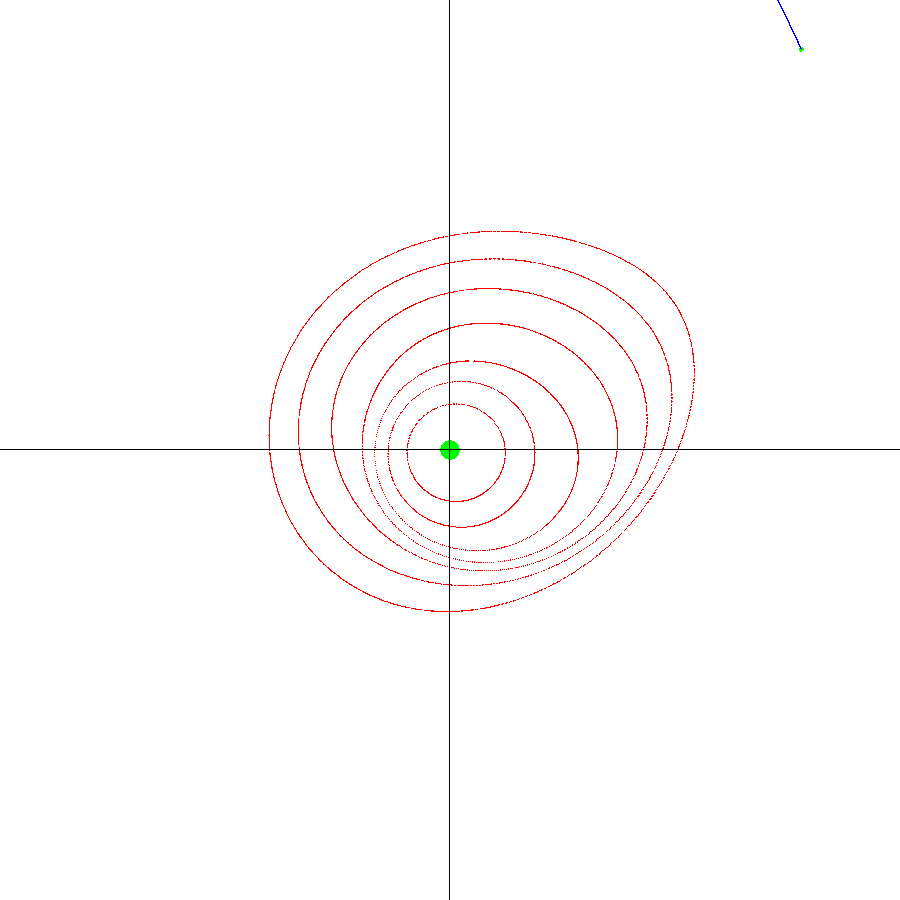
\includegraphics[width=.8\linewidth]{{../output/e-rmin-theta0-rot-1-18-0.2--1/screenshot-40.00_(-18.32_18.32)(-18.32_18.32)}.png}
  \caption{t = 40.0s}
  \label{fig9:sfig1}
\end{subfigure}%
\begin{subfigure}{.5\textwidth}
  \centering
  \includegraphics[width=.8\linewidth]{{../output/e-rmin-theta0-rot-1-18-0.2--1/screenshot-60.00_(-18.32_18.32)(-18.32_18.32)}.png}
  \caption{t = 60.0s}
  \label{fig9:sfig2}
\end{subfigure}
\begin{subfigure}{.5\textwidth}
  \centering
  \includegraphics[width=.8\linewidth]{{../output/e-rmin-theta0-rot-1-18-0.2--1/screenshot-80.00_(-18.32_18.32)(-18.32_18.32)}.png}
  \caption{t = 80.0s}
  \label{fig9:sfig3}
\end{subfigure}
\begin{subfigure}{.5\textwidth}
  \centering
  \includegraphics[width=.8\linewidth]{{../output/e-rmin-theta0-rot-1-18-0.2--1/screenshot-100.00_(-18.32_18.32)(-18.32_18.32)}.png}
  \caption{t = 100.0s}
  \label{fig9:sfig4}
\end{subfigure}
\begin{subfigure}{.5\textwidth}
  \centering
  \includegraphics[width=.8\linewidth]{{../output/e-rmin-theta0-rot-1-18-0.2--1/screenshot-120.00_(-18.32_18.32)(-18.32_18.32)}.png}
  \caption{t = 120.0s}
  \label{fig9:sfig5}
\end{subfigure}
\begin{subfigure}{.5\textwidth}
  \centering
  \includegraphics[width=.8\linewidth]{{../output/e-rmin-theta0-rot-1-18-0.2--1/screenshot-140.00_(-18.32_18.32)(-18.32_18.32)}.png}
  \caption{t = 140.0s}
  \label{fig9:sfig6}
\end{subfigure}
\caption{Plots at 6 different times (36.64 units x 36.64 units) for a perturbing galaxy with a parabolic orbit (e = 1) of closest approach 18 units and starting angle $0.2 \times 2\pi$. Test particles initially in clockwise circular orbit around central mass. (cmd-line args \{1 0.2 18 -1 1\}) }
\label{fig9:fig9}
\end{figure}
\clearpage

\begin{figure}
\begin{subfigure}{.5\textwidth}
  \centering
  \includegraphics[width=.8\linewidth]{{../output/e-rmin-theta0-rot-1-18-0.2-1/screenshot-40.00_(-18.32_18.32)(-18.32_18.32)}.png}
  \caption{t = 40.0s}
  \label{fig9:sfig1}
\end{subfigure}%
\begin{subfigure}{.5\textwidth}
  \centering
  \includegraphics[width=.8\linewidth]{{../output/e-rmin-theta0-rot-1-18-0.2-1/screenshot-60.00_(-18.32_18.32)(-18.32_18.32)}.png}
  \caption{t = 60.0s}
  \label{fig9:sfig2}
\end{subfigure}
\begin{subfigure}{.5\textwidth}
  \centering
  \includegraphics[width=.8\linewidth]{{../output/e-rmin-theta0-rot-1-18-0.2-1/screenshot-80.00_(-18.32_18.32)(-18.32_18.32)}.png}
  \caption{t = 80.0s}
  \label{fig9:sfig3}
\end{subfigure}
\begin{subfigure}{.5\textwidth}
  \centering
  \includegraphics[width=.8\linewidth]{{../output/e-rmin-theta0-rot-1-18-0.2-1/screenshot-100.00_(-18.32_18.32)(-18.32_18.32)}.png}
  \caption{t = 100.0s}
  \label{fig9:sfig4}
\end{subfigure}
\begin{subfigure}{.5\textwidth}
  \centering
  \includegraphics[width=.8\linewidth]{{../output/e-rmin-theta0-rot-1-18-0.2-1/screenshot-120.00_(-18.32_18.32)(-18.32_18.32)}.png}
  \caption{t = 120.0s}
  \label{fig9:sfig5}
\end{subfigure}
\begin{subfigure}{.5\textwidth}
  \centering
  \includegraphics[width=.8\linewidth]{{../output/e-rmin-theta0-rot-1-18-0.2-1/screenshot-140.00_(-18.32_18.32)(-18.32_18.32)}.png}
  \caption{t = 140.0s}
  \label{fig9:sfig6}
\end{subfigure}
\caption{Plots at 6 different times (36.64 units x 36.64 units) for a perturbing galaxy with a parabolic orbit (e = 1) of closest approach 18 units and starting angle $0.2 \times 2\pi$. Test particles initially in anticlockwise circular orbit around central mass. (cmd-line args \{1 0.2 18 1 1\}) }
\label{fig9:fig9}
\end{figure}

\clearpage
\section{Instructions}
\subsection{Building and Running}
Software Required:
\begin{enumerate}
\item C++ compiler ( C++11 compliant)
\item SDL2
\item OpenGL
\item GLEW
\item cmake
\end{enumerate}

Instructions:

\begin{lstlisting}
	cd {project-directory}
	cmake .
	make
	cd bin
	./main {command-line-arguments}
\end{lstlisting}
\textbf{Command line arguments:} 5 arguments supplied (Eccentricity, $\theta_0$, Closest Approach, Rotation direction of central galaxy ($-1=\circlearrowright, 1=\circlearrowleft$), Perturbation orbit direction).
\\
\\
\textbf{Command line arguments:} 4 arguments supplied (Eccentricity, $\theta_0$, Closest Approach, TESTING (1 = true, 0 = false))
\\
\\
\textbf{Command line arguments:} 1 argument supplied (INTERACTIVE (1 = true, 0 = false))
\\
\\
Other combinations result in a default simulation being carried out.
\\
\\
\textbf{Logging Information:} Each time step is output to a new line in the data file so that each line has the format t,\{x1,y1,z1\},\{x2,y2,z2\},...,\{xN,yN,zN\}. A Python script could easily be created to carry out text processing on this data file to extract all of the particle's positions at a specific time. The extracted positions could then be written to a text file in a plot friendly format i.e. x1,y2 \{newline\} x2,y2 etc. and then plotted (matplotlib) all within the same script. This script was not created as it was felt that the screenshots provided sufficient graphical information.

\subsection{Controls}
\begin{itemize}
\item Pan - WASD $(\uparrow \leftarrow \downarrow \rightarrow)$.
\item Zoom out/in - QE $(-+)$.
\item Take Screenshot - P (screenshots are automatically taken at 5.0s intervals (simulated system time)) (.tga file created, can be converted with convert\_png.sh script provided).
\item Start/Stop data logging to .csv - L.
\item Start/Pause/Unpause - SPACEBAR.
\item INTERACTIVE == true - left click, drag then release to create a massive particle with velocity proportional to length and direction of drag.
\end{itemize}

\clearpage
\newgeometry{left=1.0cm,bottom=2cm}
\section{Code Listings}
\subsection{radius\_plot.p}
\lstinputlisting{../bin/radius_plot.p}
\subsection{convert\_png.sh}
\lstinputlisting{../bin/convert_png.sh}
\subsection{sdl\_guard.h}
\lstinputlisting{../include/utilities/sdl_guard.h}
\clearpage
\subsection{main.cpp}
\lstinputlisting{../src/main.cpp}
\clearpage
\subsection{logger.h}
\lstinputlisting{../include/capture/logger.h}
\subsection{logger.cpp}
\lstinputlisting{../src/capture/logger.cpp}
\clearpage
\subsection{screenshot.h}
\lstinputlisting{../include/capture/screenshot.h}
\subsection{screenshot.cpp}
\lstinputlisting{../src/capture/screenshot.cpp}
\clearpage
\subsection{particle.h}
\lstinputlisting{../include/physics/particle.h}
\subsection{particle.cpp}
\lstinputlisting{../src/physics/particle.cpp}
\clearpage
\subsection{universe.h}
\lstinputlisting{../include/physics/universe.h}
\subsection{universe.cpp}
\lstinputlisting{../src/physics/universe.cpp}
\clearpage
\subsection{camera.h}
\lstinputlisting{../include/utilities/camera.h}
\subsection{camera.cpp}
\lstinputlisting{../src/utilities/camera.cpp}
\clearpage
\subsection{utilities.h}
\lstinputlisting{../include/utilities/utilities.h}
\subsection{utilities.cpp}
\lstinputlisting{../src/utilities/utilities.cpp}


\end{document}